% !TEX root = ../main.tex

\chapter{Patanalysis}
\label{ch:analysis}

\startcontents[chapters]

\vfill

Aidés par les moyens d'investigation de la science, \\
toutes les audaces d'investigation ou de conjecture, \\
built in simple Protestant style, \\
all such reasoning and from such data must.

And I style him friend, \\
its whole style differed materially from that of Legrand, \\
the calculus of Probabilities, \\
n'échappaient à leur investigation.

Another line of reasoning partially decided me, \\
to make an anatomical dissection of its body and, \\
ce style en débâcle et innavigable.

In a style Of gold, \\
que la sobriété du style se conduit de la sorte, \\
still a point worthy very serious investigation.

\newpage
\minicontents
\spirals

\section{Opinions}

% \section{Creativity Focus Group}

Sunday 03 January 2016

\begin{itemize}
  \item Sally - artist, teacher
  \item Paul - gardener
  \item Henrietta - artist
  \item Jonathan -
  \item Dave - programmer, musician, writer, artist, lecturer
\end{itemize}

\url{http://sallywilsonprints.com/}
\url{http://henriettacorbett.co.uk/}
\url{http://daveeveritt.org/}

0:04 J: It's about this thing about being ... by all the restrictions, you know we are all very ...? We are all ... via structures, by things that have happened in our lives, by upbringing, by school, by friends, by conventions, by norms. Free yourself out of that, and come out of it - that's when you can be truly creative. You don't, might not know what that actually means. You've got the energy of being creative and that's when, once you've decided maybe what you wanna do maybe, that's when this form comes through... that's how I see it.

0:34 S: What's the trigger then, for making you change from how you are every day?

0:38 F: I think, it's because you're, well, what you're saying is that you need to let go of those constraints and restrictions...

0:44 J: Yeah, yeah, absolutely.

0:45 F: but it is an acknowledgement of the constraints that then triggers the creativity.

0:50 J: Yeah.

0:52 H: What I think that you're missing, is that you cannot be wholly creative if you haven't got some sort of process to follow to engage your creativity

1:05 J: I already acknowledged that, but

1:06 H: It's all very well to throw clay around or paint around if you have no process to work towards.

1:12 J: I already acknowledged that has to happen in order create something with .... for example... but to answer the question of what's creativity .......... 1:24 but creativity per se for me its letting go of all the shackles, everything you've learned maybe ....

1:34 S: You say that, but how do you do that?

1:34 ?: You've got no reference points...

.....

1:42 D: I think what you mean is that there are constraints that act on you that can stifle your creativity.

1:49 S: How, where's the switch, that changes that?

1:55 D: You need some kind of method, some kind of approach to channel that.

...

2:06 D: So it's constraints that you haven't chosen that stifle it and constraints that you have chosen..?

2:12 J: It's the process that H is talking about is .... a process of channeling that creativity to some kind of conclusion.

2:18 P: Are you in control of the process though?

2:22 S: The process is the creative part.

2:24 P: Does the process lead you to a different place?

2:35 S: You can sit and think I'm going to create this, that and the other. When you actually come down to it, when you're handling the materials something else happens. Because the materials and the process are involved in the outcome. It's not an intellectual idea.

2:53 J: The creativity can drive the process. How many artists ... start of writing or doing a piece of art.... they don't have a clue, they have no idea what they're gonna do. But all of a sudden ...it goes into completely different directions, completely, that's creativity. You don't start off with a process. You don't know how exactly .....

3:31 D: How does that swerve happen? You know when you're doing something, and suddenly it starts to take on a life of it's own.

3:43 H: A stone carver sits there with a lump of stone, the immediate moment he starts his first chip, he's doing a process. He's following a process with tools. It's both at the same time. Creativity is taking over and a process, all at the same time. Because without the process there is no, you can't just bash into it and see what happens. you know, the tool and the knowledge, all those things have come together to make you be able to be creative. And the more knowledge you've got, and the more processes you know the more creative you can be. So one doesn't stifle the other.

4:24 J: I think we are looking at two different ways of describing, well we obviously are but, ...

4:36 H: You're talking about an emotional freedom aren't you?

4:50 J: Everyone's creative, it's just finding you're creativity, I guess. I mean a little child is creative, play with a bit of paper and create something, they're not going through a process of creating... that takes some kind of consciousness, some intellectual ...

5:03 S: Children are naturally creative but that is taken out of them at quite an early age now because of our school system.

5:10 J: Well, again, because of the things that are put in place to restrict you maybe.

5:17 D: How would you define those constraints? Could you label them?

5:23 J: Well, as I said before, they could be as simple as upbringing, society, the way we conform to society, the way we conform to convention, the way we conform to the way of thinking, you know, a lot of these so called creative geniuses for example, are people who've destroyed the norms, they've looked outside the box, they've done that.

5:43 H: Well, those people have had time. What you're talking about is, people like yourself haven't had time to be creative, haven't had the freedom of time to be creative because you've gone down a path of work, commuting, driving, office, all those things you're doing that for you salary. You know, in the big scheme of things, the majority of public do that in this country to earn a living. Creativity is squashed out of them because of time. you know, they've got constraints of family, having to do the cleaning, the washing the ironing, getting the tea and all the rest of it, so creativity so squashed out. so anytime they would consider being creative is if they signed up to an evening class, you know, in the evening where you're time limited again. But if you took jobs away and you took responsibilities away and you allow people to just to, if they had money and all the rest of it, and they didn't work and then you find a lot more people would probably want to be creative. because they would think of i can do that or i can do that.

6:54 D: Yeah, I agree, but I'm not sure that time constraints are everything.

7:09 P: [Baboon story]

8:39 S: I've you've got all those security things you can then ...

8:44 H: So if everything is placed before you so you've got no demands made on you, then, I think partially that is about time. Well, its about time when we look at our society but because our time is taken up providing for ourselves and providing for others, but if you take that away, if everything is provided for you, and fear is taken away form you, then you play. because thats whats left.

9:15 S: Thats a very key thing.

9:21 H: So then you're creative, when you play. I think play is a natural human thing. But we don't get to do it very much, well I do, because i get to do it for my job quite often. I make enormous amounts of mistakes, which you learn from. there will come a time when play is no longer enjoyable, if you haven't got a process to further the play. so that things stay together and build.

9:52 F: Can I ask you what you think how to evaluate creativity? If you look at a piece of art, and you're asked to judge, you know, give it, on a scale of 1 to 10, say how creative is this? What are the attributes or factors that you would take into account in order to judge a piece of art?

10:12 J: Just be an emotional one. Emotional response.

10:19 P: I'd have to understand how the piece came together. I'd have to know its history.

10:27 H: Well, theres an inventiveness that i'd look for. There a part of emotion that comes into it. Inventiveness, cleverness, technique, all those things that...

10:37 S: If it makes me think, or if it's life enhancing,

10:42 H: That's an emotional response.

10:43 J: Hm, that's an emotional response, yeah.

10:47 H: Yeah, I think it's the inventive quality I think that

11:15 S: It takes you away from the everyday things in life and makes you go into a more thoughtful world. It's reflective, which our society doesn't really do. For me, that reflective thing...

11:38 H: Inventiveness, creativity.

11:39 F: Do you think we can measure creativity objectively?

11:45 P: Only if you know the context in which it took place I feel.

11:47 S: I don't think you can measure it as you can measure other things.

12:08 D: So how do art administrators evaluate work that their funding?

12:13 P: Maybe they don't, we just think they do.

12:18 D: Because theoretically, if what you say is true, we can't measure...

12:21 S: Is it interesting, is it challenging?

12:22 H: It can measure quality.

12:24 D: How?

12:24 F: How do you measure quality? In an art work?

12:26 J: Do you mean skill? That sort of thing? Ability?

12:30 S: It's skill but also, is it thoughtful?

12:34 F: Yeah but what makes skill in terms of art? If you think of

12:37 J: Technique.

12:40 F: What makes this kind of brush stroke more skillful than another kind of brush stroke.

12:45 S: Its the whole thing, its not a question of the brush stroke. Because you can take a Van Gogh painting and you can split it up into its bits, but it still will not be what the whole thing is.

12:56 D: If you copy it, would that be creative?

13:01 S: No what I'm saying is that you can split it up, but it wont have that defining thing about it. If you put it all together its a Van Gogh painting.

13:06 H: If you copied it, completely to the nth degree

13:11 S: It would mean nothing.

13:11 F: It's not inventive.

13:13 H: It's not inventive, therefore its not creative. The inventive word is quite a strong word.

13:18 J: Again, because you've got no emotional investment in it. You know, its not yours.

13:24 H: There is no emotion.

13:24 S: Its not the sum of its parts, its something else.

13:29 P: This is the talent.

13:31 H: Clever, technique.

13:33 D: Yeah, theres a lot of difference between technique and creativity.

13:42 S: Grayson Perry said the most interesting thing: He said: ``Creativity is an accident.'' What you have to do is to set up a situation where that accident can happen. That's to do with process. Thats to do with knowing about your materials, knowing how to manipulate paint or whatever, or printmaking, and then seeing what happens. But you can't do it, It's like the intellect and intuition coming together.

14:05 P: But, if you ask somebody to draw a milk bottle when they're feeling cheerful, here comes the page, they're starting to draw or paint a milk bottle, they're gonna paint a milk bottle. fair enough. you stress that person out, ask the person to draw the same milk bottle and in a different frame of mind, you're gonna get a different milk bottle. you know, if somebody is really peeved and pissed off they might smash that bottle. where is the technique evaluation on that because the smashed bottle actually says a lot equally.

14:36 H: Its an emotional response.

14:42 P: Yeah I suppose it is yeah.

...

15:10 P: There's what the person's experiencing and

15:13 S: No, but you're talking about the object itself, what you're asking is we are judging the object. Doesn't matter if we know anything about the artist.

15:26 F: Do you need to know about the process in order to judge a piece of artwork.

15:31 H: I think so.

15:31 J: In order to judge it critically maybe, but not to judge it emotionally. That's a difference , isn't it. If I look at a painting, first of all, do I like it? Do I like it? And then I'll go up to it

15:43 F: Funding bodies, you know, if they're asked to give money to artists, they cant rely on their emotional judgement.

15:52 P: They have to make a snap decision based on intuition. They look at it and know.

15:57 D: They don;t. They have a list, they have a checklist.

15:58 H: They have a list of tick boxes.

16:00 J: That's how critics make their living. They just go and be critical.

16:10 J: The public, they either like it or don't. They don't go round really thinking about how its all done.

16:15 S: But somebody has to judge these ...

[...]

16:56 H: Tick boxes.

17:00 D: But then also, the critics and art funders do tend to shape culture by supporting things, and that support gains a momentum, and everything outside of that support momentum gets marginalised.

17:14 H: Side lined.

17:16 J: They've got a lot to answer for.

17:18 D: And then some marginalised things like digital art where marginalised until like 10 years ago.

17:22 J: And they're hugely influential.

17:23 D: Yeah, now its now they can do anything. But that tide of evaluation of ``this is of worth'' ``this is not of worth'' that shifts.

17:35 S: Yeah because they are, like Pamela Clarkson said: ``Paintings are completely out of fashion''. It's not, it's coming back now. You'd be a fool as an artist of you follow fashion.

17:51 F: I was just thinking that ... if a computer is being creative its not really being creative its the programme that's being creative. but in a sense if you look at well, ... I thought we can look at programming and computer art , if you look at it as a tool, like a visual artist would use a brush and paint.

18:20 D: It's the same thing. Its just a medium.

18:28 S: What are you expecting from your computer?

18:32 F: That's the question I think. I think Im trying to answer the question of whether well, for starters i'm saying that its not the computer itself, the computer is just a tool. or specific technique. so you need to look at the context , the programmer, the background of the programmer , the cultural background of the programmer, and all of these things in order to judge a creative output by the computer.

19:03 H: The computer needs a human.

19:05 F: Yeah.

19:09 S: How can you have a creative output from a computer?

19:07 H: with a human intervention.

19:11 D: With tools, its just a tool. So its the same as any other tool. Art technology has been going on for a long time, when painters mixed their own pigments. they had to learn chemistry and all sorts of other bits and pieces.

19:23 S: But however much a computer learned it couldn't learn to get it wrong.

19:29 D: No, but the programmer.

19:32 S: But could it learn to get it wrong.

19:36 F: It could. If you identify ,you know, if you now say that playing with these mistakes and errors is part of your creative process, then you could teach theoretically you could write routines that tell the computer to experiment with their parameters

19:56 S: But how would the computer know when it wasn't right?

20:01 F: Well, the same way you, how do you know something is right or wrong.

20:04 S: Because i'm a human being.

20:05 P: yeah but you'd have to be developing the computers consciousness, then you would be the means by which that computer is starting to develop basic level of consciousness. because thats a counter point, knowing you got something wrong, means you have had an idea beforehand. what it needed to be. thats the development of consciousness.

20:21 D: That's the problem.

20:23 S: How would a computer know if it was right?

20:24 H: It cant just all be random can it?

20:34 F: Essentially thats what i'm doing with pataphysics. i'm using that as a way of introducing sort of pseudo randomness into

20:39 H: yeah, and pseudo emotion. cause its emotional response...

20:47 S: Why is it desirable for a computer to be creative?

20:52 F: I don't think..., i don't know. Its a good point. I think its just the way humanity goes, technology

21:00 D: Thats not the question. Its just another tool.

21:04 J: Exactly.

21:08 S: Yeah but why would be want computers to emulate a human response?

21:12 J: Thats not the question though.

21:13 F: thats like asking why do we want computers to be intelligent. its the same question.

21:19 S: Why do we? why cant we just have another tool?

21:27 P: Because the nature of evolution, evolution is on every level its not just about flesh and blood. evolution is on every level and in every way and every technique. its part of the evolution of gr....

21:39 D: When you use Google and you type in a load of words, and you expect a result that makes sense, thats the computer being programmed to be intelligent on your behalf.

21:51 S: Why do you want it to take over the human attributes?

21:52 D: It doesn't. It just aids you. its like, the internets big, so if you type in ``cute cat video'', you want to make sure you're gonna get cute cat videos.

22:19 S: The computer is great at getting those cats but its great as a tool but never gonna beat the human mind.

...

22:48 S: Its just interesting, why do people want the computer to emulate the human brain. because the human brain has got so much weirdness and errors and strange things about it.

22:55 D: Thats exactly why. Its about finding out about ourselves.

23:01 F: This is a strand. AI has two strands in a sense. One is they're studying human brains and computers because they're trying to understand the human brain. but the other is

23:12 S: Computers are based on the binary system. Our brains aren't based on the binary system. they aren't yes and no.

23:20 F: Actually you could argue that they're dead and alive.

23:24 D: DNA is completely binary. Life is binary.



\section{Problems Encountered}

% \begin{draft}
%   \section{User experience}
%
%   Whilst developing a system that returns creative results to the end user has numerous advantages, the assumptions that are made about and the decisions we take for the user must still be considered. For example, presume that the user inputs a search request `The Cat in the Hat' after reading a Dr.\ Seuss book to their child, and the system employs an anomalous method on the query and searched `sunglasses'. Whilst there is logic to the new search request, it is anomalous to the initial request, if the user receives these results without being told what method was used, the results will appear random, and therefore are likely to be detrimental to the user. Therefore the level of interaction the user has with the system and the feedback the system gives to the user on decisions it is making will have a large influence on the overall effectiveness and appreciation of the search tool. A quick and simple solution to this problem would be to add an icon to the side of each search result which displays how the original query was pataphysicalised.
%
%   \begin{figure}[htb] % (here, top, bottom, page)
%     \centering
%     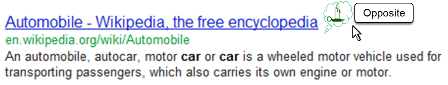
\includegraphics[width=\linewidth]{images/resultexample}
%   \caption[Feedback button]{Feedback button}
%   \label{fig:feedback}
%   \end{figure}
%
%   The above image (figure~\ref{fig:feedback}) shows an example of how this could be implemented. The little green candle (a reference to pataphysics in itself by the way) shows a pop-up note when hovered over with the mouse pointer. In this case the original query could have been `tree' and `car' was returned as an opposite to that.
% \end{draft}


\section{Design Aspects}

\section{Search Results}

\stopcontents[chapters]
